% Grid event or data artefact? -- manuscript for Applied Energy (Elsevier, elsarticle class).
% Build: latexmk -pdf main.tex   (or pdflatex, bibtex, pdflatex, pdflatex). Word count: python tools/wordcount.py
% Rules for every sentence: numbers only from docs/results_summary.md; references only from verified DOI metadata
% (paper/README.md). Figures are copied to figures/ as Figure_N.pdf by tools/sync_figures.py.
\documentclass[preprint,12pt]{elsarticle}

\usepackage[T1]{fontenc}
\usepackage[utf8]{inputenc}
\usepackage{amsmath,amssymb}
\usepackage{graphicx}
\usepackage{booktabs}
\usepackage{array}
\usepackage{tabularx}
\usepackage{lineno}
\usepackage{xcolor}
\usepackage[hidelinks]{hyperref}

\graphicspath{{figures/}}
\newcolumntype{L}[1]{>{\raggedright\arraybackslash}p{#1}}
\newcolumntype{Y}{>{\raggedright\arraybackslash}X}

% notation used throughout
\usepackage{dsfont}
\newcommand{\xh}{\hat{x}}
\newcommand{\one}{\mathds{1}}   % indicator function

\journal{Applied Energy}

\begin{document}

\begin{frontmatter}

\title{Grid event or data artefact? Hierarchical weak supervision for anomaly attribution in multi-city feeder telemetry}

% Authors, affiliations and the corresponding author are added by the author (title-page rules in paper/OUTLINE.md).
\author[a]{[Author names to be added]}
\affiliation[a]{organization={[Affiliation to be added]},
                country={Morocco}}

\begin{abstract}
[Written last: at most 250 words; purpose, procedures, main findings with their statistical significance, principal conclusions.]
\end{abstract}

\begin{keyword}
weak supervision \sep anomaly attribution \sep feeder telemetry \sep data quality \sep outage statistics \sep load forecasting \sep distribution networks
\end{keyword}

\end{frontmatter}

\linenumbers

% Introduction -- budget 850 words. Plan (paper/OUTLINE.md): 1.1 motivation; 1.2 the problem; 1.3 gap (verified references); 1.4 contributions V1-V5 + catalogue; 1.5 RQ1-RQ5, H1-H3; 1.6 organisation. Written in step 9.
\section{Introduction}\label{sec:intro}

[To be written.]

% Related work -- budget 850 words. Plan (paper/OUTLINE.md): 2.1 load anomaly detection; 2.2 physical events vs data-quality faults; 2.3 weak supervision; 2.4 multivariate and graph time-series detection; 2.5 evaluation; 2.6 positioning + Table 1. Written in step 8.
\section{Related work}\label{sec:related}

[To be written.]

% Data, hierarchy and typology -- budget 850 words (body text).
% Sources: results/paper/tables/Table1_data_inventory.csv, Table2_typology.csv; docs/methods.md section 1;
% docs/results_summary.md; external facts from bensalah2025dib (full text read) and the UCI records.
\section{Data, hierarchy and typology}\label{sec:data}

\subsection{Datasets}\label{sec:datasets}

The study uses the UCI high-resolution load dataset from smart meters in four Moroccan cities \cite{bensalah2025uci,bensalah2025dib}, introduced with a load-forecasting study \cite{bensalah2025opsearch}. The meters are installed by the national utility ONEE on 22~kV distribution feeders and record at 10-min intervals (30~min in Marrakech); the data were exported manually from the meters \cite{bensalah2025dib}. In Laâyoune, Boujdour and Foum El Oued the dataset covers every 22~kV feeder departure \cite{bensalah2025dib}, so each city is observed in full. Each feeder is a \emph{zone} in the dataset's terminology.

Table~\ref{tab:data} lists the series. The three southern cities (15 zones, in amperes) share one 10-min timeline from 14 September 2022 to 24 May 2024, with the same 12 missing time stamps in every zone. We call them the \emph{southern system}; it carries most of the analysis. Marrakech (2 zones, in kW, 2023) is recorded on its own 30-min timeline and is treated as a separate system. The UCI Tetouan dataset \cite{salam2018uci,salam2018irsec}, three distribution networks of one city at 10-min steps in 2017, is used only to test transfer to a new system (Section~\ref{sec:results}). Fig.~\ref{fig:data}(a) locates the five cities.

None of the datasets comes with event labels: there is no record of which zeros or flat stretches are outages and which are acquisition failures. Exact zeros alone occupy 7,201 zone-steps in the southern system (Table~\ref{tab:data}). All time stamps are used as recorded, without any clock correction, so that clock errors remain observable as a data property.

\begin{table}[t]
\centering
\caption{Datasets. Regular steps: length of the regular time grid from the first to the last stamp. Missing steps: grid steps without a record. Zone-steps: one zone at one time step.}
\label{tab:data}
\footnotesize
\setlength{\tabcolsep}{4pt}
\begin{tabularx}{\textwidth}{@{}l c c c Y r r r@{}}
\toprule
City & Zones & Step & Unit & Period & Regular & Missing & Exact-zero \\
     &       & (min) &     &        & steps   & steps   & zone-steps \\
\midrule
Laâyoune     & 5 & 10 & A  & 14 Sep 2022 -- 24 May 2024 & 88,890 & 12 & 1,465 \\
Boujdour     & 3 & 10 & A  & 14 Sep 2022 -- 24 May 2024 & 88,890 & 12 & 1,413 \\
Foum El Oued & 7 & 10 & A  & 14 Sep 2022 -- 24 May 2024 & 88,890 & 12 & 4,323 \\
Marrakech    & 2 & 30 & kW & 9 Jan 2023 -- 8 Jan 2024   & 17,520 & 25 & 101 \\
Tetouan$^{a}$ & 3 & 10 & n.s. & 1 Jan 2017 -- 30 Dec 2017 & 52,416 & 0 & 0 \\
\bottomrule
\end{tabularx}

\vspace{2pt}
\footnotesize{$^{a}$Transfer test only. n.s.: unit not stated in the repository record \cite{salam2018uci}.}
\end{table}

\begin{figure}[t]
\centering
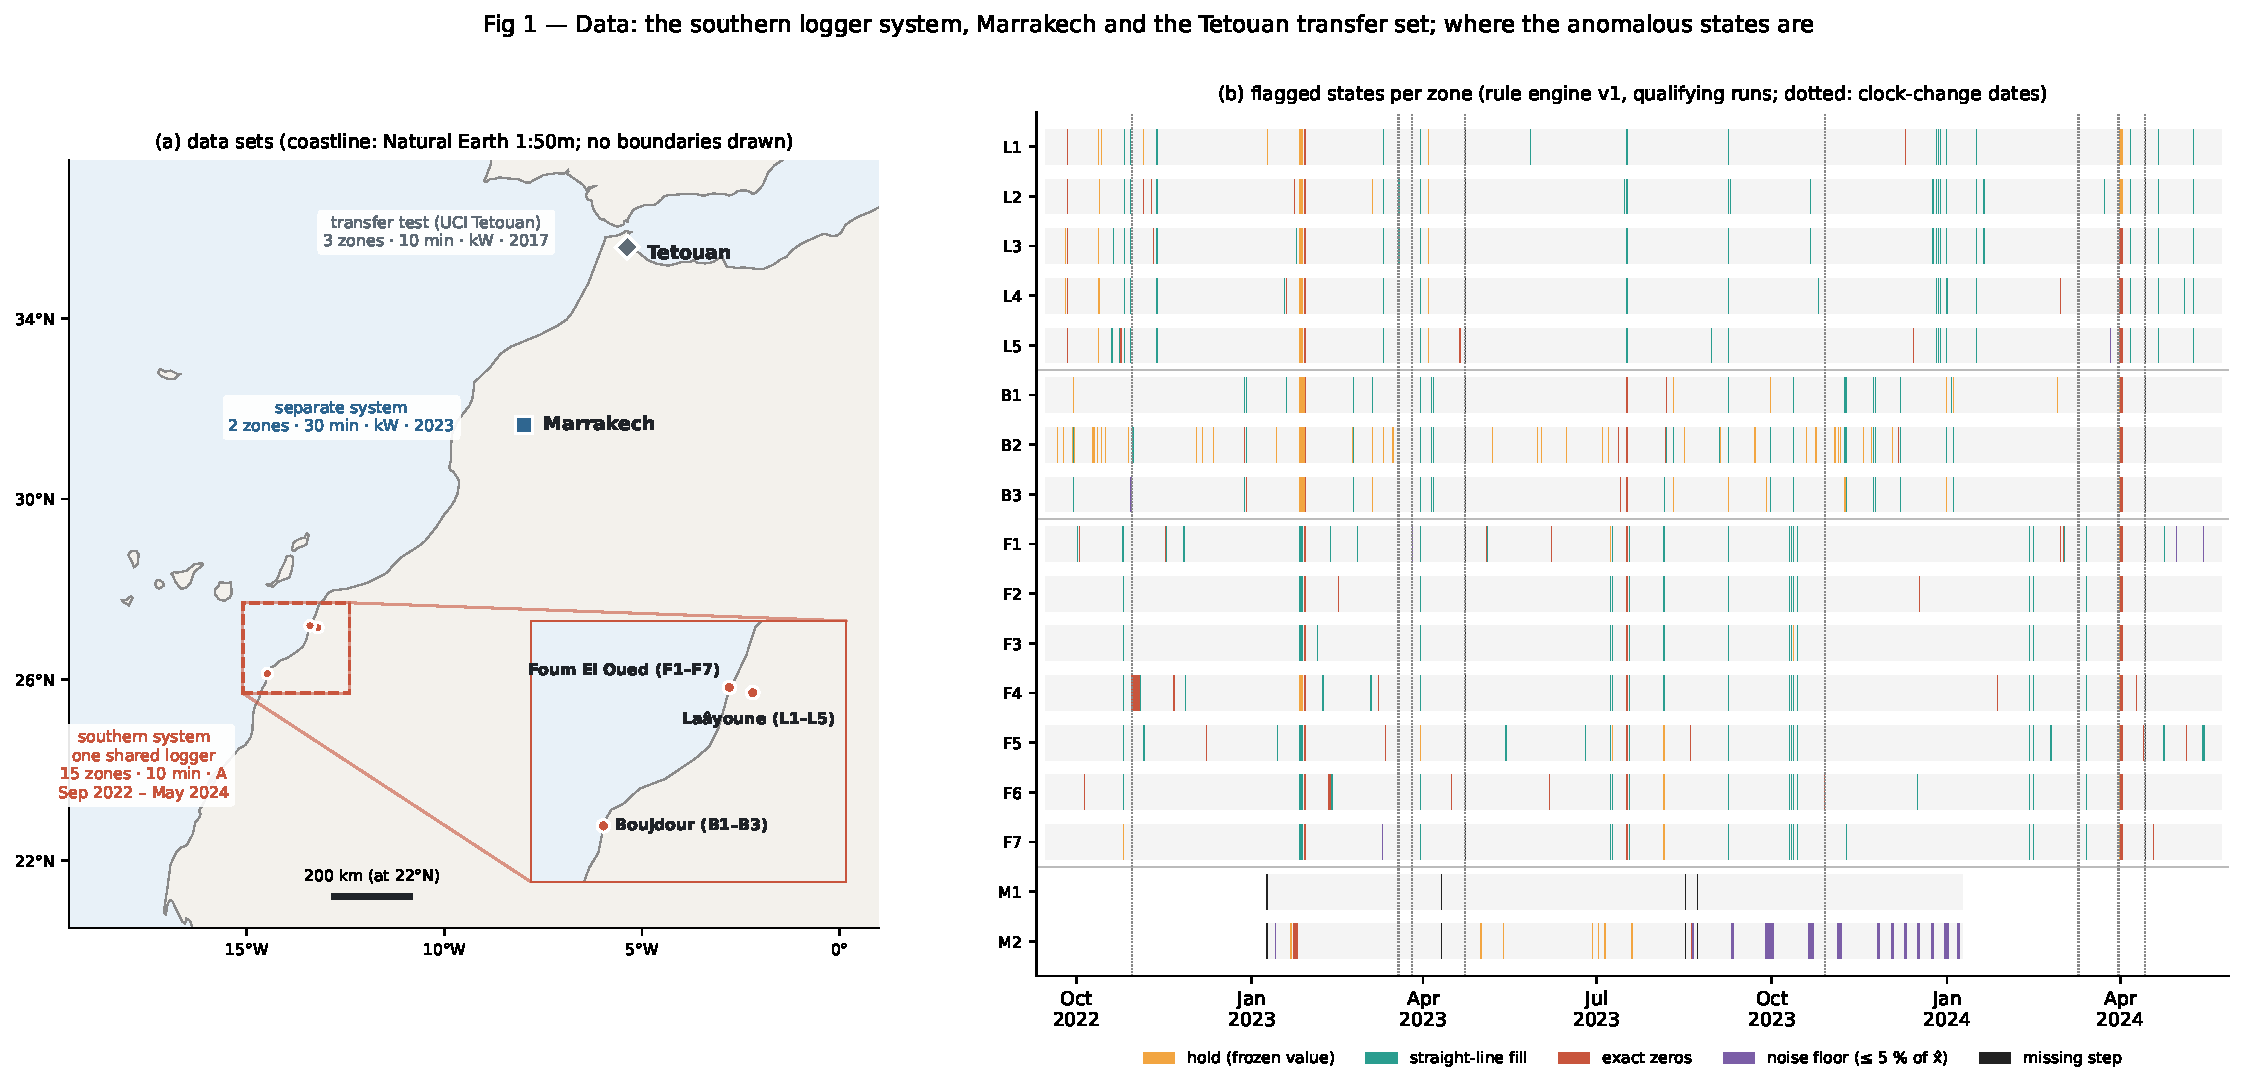
\includegraphics[width=\textwidth]{Figure_1}
\caption{Data. (a) The five cities. Laâyoune, Boujdour and Foum El Oued (15 zones, 10~min, A) share one recording timeline; Marrakech (2 zones, 30~min, kW) is a separate system; Tetouan (3 zones, 2017) is the transfer test. Coastline from Natural Earth (1:50m, public domain); no boundaries are drawn. (b) Anomalous states per zone (holds, straight-line fills, exact zeros and noise-floor runs of qualifying length, and missing steps; Section~\ref{sec:method}); dotted lines mark clock-change dates. Time stamps as recorded.}
\label{fig:data}
\end{figure}

\subsection{The telemetry hierarchy}\label{sec:hierarchy}

The southern series form a three-level hierarchy: zone (one feeder), city (all feeders of one city) and region (the three cities). Each level corresponds to a different cause of a disturbance. A feeder fault or planned maintenance affects one zone. Losing a city's supply point de-energises all of that city's zones while the other cities keep running. A regional event affects several cities at once.

The acquisition chain forms a fourth, non-electrical layer. The three cities are recorded on one timeline, and a failure in the shared recording or export process can hit zones in different cities at the same time step, regardless of the electrical topology. Such a failure also leaves traces that a de-energised feeder does not: series held at an identical value, stretches that are perfectly straight lines, and exact zeros where a de-energised feeder often reads a small, noisy residual current. The method uses these signatures together with the level at which an anomaly appears: simultaneity across cities, combined with these traces, is evidence of an artefact, whereas a noise floor confined to one zone or one city is evidence of a grid event.

\subsection{Problem formulation}\label{sec:problem}

Let $x_{z,t}$ be the recorded value of zone $z$ at time step $t$, and $P$ the number of steps per day (144 at 10~min, 48 at 30~min). The expected value is the median of the same time-of-day slot over the previous $K = 14$ days, excluding zeros:
\begin{equation}
\xh_{z,t} = \operatorname{median}\left\{ x_{z,t-kP} \;:\; k = 1,\dots,K,\; x_{z,t-kP} \neq 0 \right\}.
\label{eq:expected}
\end{equation}
The relative level
\begin{equation}
\rho_{z,t} = x_{z,t}/\xh_{z,t}
\label{eq:rho}
\end{equation}
is unit-free, so amperes, kilowatts and feeders of different sizes are compared on one scale.

An anomalous \emph{item} $i$ is a time span with a set of affected zones. Its type $y_i$ belongs to $\mathcal{Y} = \{\mathrm{A1},\dots,\mathrm{A4},\mathrm{G1},\dots,\mathrm{G5},\mathrm{N}\}$ (Section~\ref{sec:typology}). The task has four parts: \emph{detection}, finding the items; \emph{attribution}, estimating a probability distribution $p_i(y)$ over $\mathcal{Y}$ for each item; \emph{localisation}, identifying the level (zone, city or region) that carries the anomaly; and \emph{type-aware cleaning}, imputing artefacts while keeping grid events in the data and marking them. All four must be solved without labelled examples.

\subsection{Typology}\label{sec:typology}

Table~\ref{tab:typology} and Fig.~\ref{fig:typology} define nine anomaly types, each with a measurable signature at one level of the hierarchy. The four \emph{data artefacts} are zero-fill gaps across cities (A1), simultaneous fills of several zones by held values or straight lines (A2), the same fills in a single zone (A3), and clock errors that shift the daily profile after a clock-change date (A4). The five \emph{grid events} are regional outages (G1), city outages (G2), unplanned feeder outages (G3), planned work (G4) and load transfers between feeders (G5). Items that match no anomalous pattern are labelled normal (N).

Straight-line fills were not part of the initial typology. They appeared in the data audit (Section~\ref{sec:results}) and are now part of A2 and A3. The expected signatures of grid events, in particular gradual restoration and cold-load pick-up after an outage, are hypotheses that Section~\ref{sec:results} tests on the real data.

\begin{table}[t]
\centering
\caption{Typology. Level: the level of the hierarchy at which the signature appears. Rules: the labelling rules that vote for the type (Section~\ref{sec:method}). Real items: rule items assigned the type in the final catalogue of the real data. $\eta$: share of exact zeros in a dead run; $\pi$: restoration overshoot; $\delta^*$: estimated clock offset; $\kappa$: conservation index.}
\label{tab:typology}
\footnotesize
\setlength{\tabcolsep}{4pt}
\begin{tabularx}{\textwidth}{@{}l L{2.1cm} L{1.9cm} Y L{1.6cm} r@{}}
\toprule
Type & Name & Level & Signature & Rules & Real items \\
\midrule
A1 & Zero-fill gap & Region ($\geq 2$ cities) & Exact zeros ($\eta = 1$) in $\geq 2$ cities at once, often after a hold or straight-line fill; returns at once & R1, R3, R4, R21 & 3 \\
A2 & Simultaneous fill & $\geq 2$ zones & $\geq 2$ zones held at identical values or straight-line interpolated over the same span & R2, R19 & 57 \\
A3 & Single-zone fill & Zone & One zone held or straight-line interpolated while its neighbours move normally & R12, R20 & 98 \\
A4 & Clock error & System, one day & Daily profile shifted by $\delta^* \approx \pm 60$~min after a clock-change date; duplicated or missing stamps & R13, R14, R15 & 14 \\
\midrule
G1 & Regional outage & Region ($\geq 2$ cities) & Noise floor ($\eta < 0.9$) in $\geq 2$ cities; gradual restoration with cold-load overshoot $\pi \geq 1.15$ & R5, R6, R7 & 0 \\
G2 & City outage & City & All zones of one city at the noise floor while the other cities stay normal & R8 (R5, R6) & 1 \\
G3 & Unplanned feeder outage & Zone & One zone at the noise floor at any hour, possibly for more than 24~h & R9, R11 (R6) & 52 \\
G4 & Planned work & Zone & One zone at the noise floor, starting 06:00--11:59, shorter than 6~h & R10 & 70 \\
G5 & Load transfer & $\geq 2$ zones of a city & One zone steps down while another steps up by the same amount ($\kappa \approx 0$) & R16 & 1 \\
\bottomrule
\end{tabularx}
\end{table}

\begin{figure}[t]
\centering
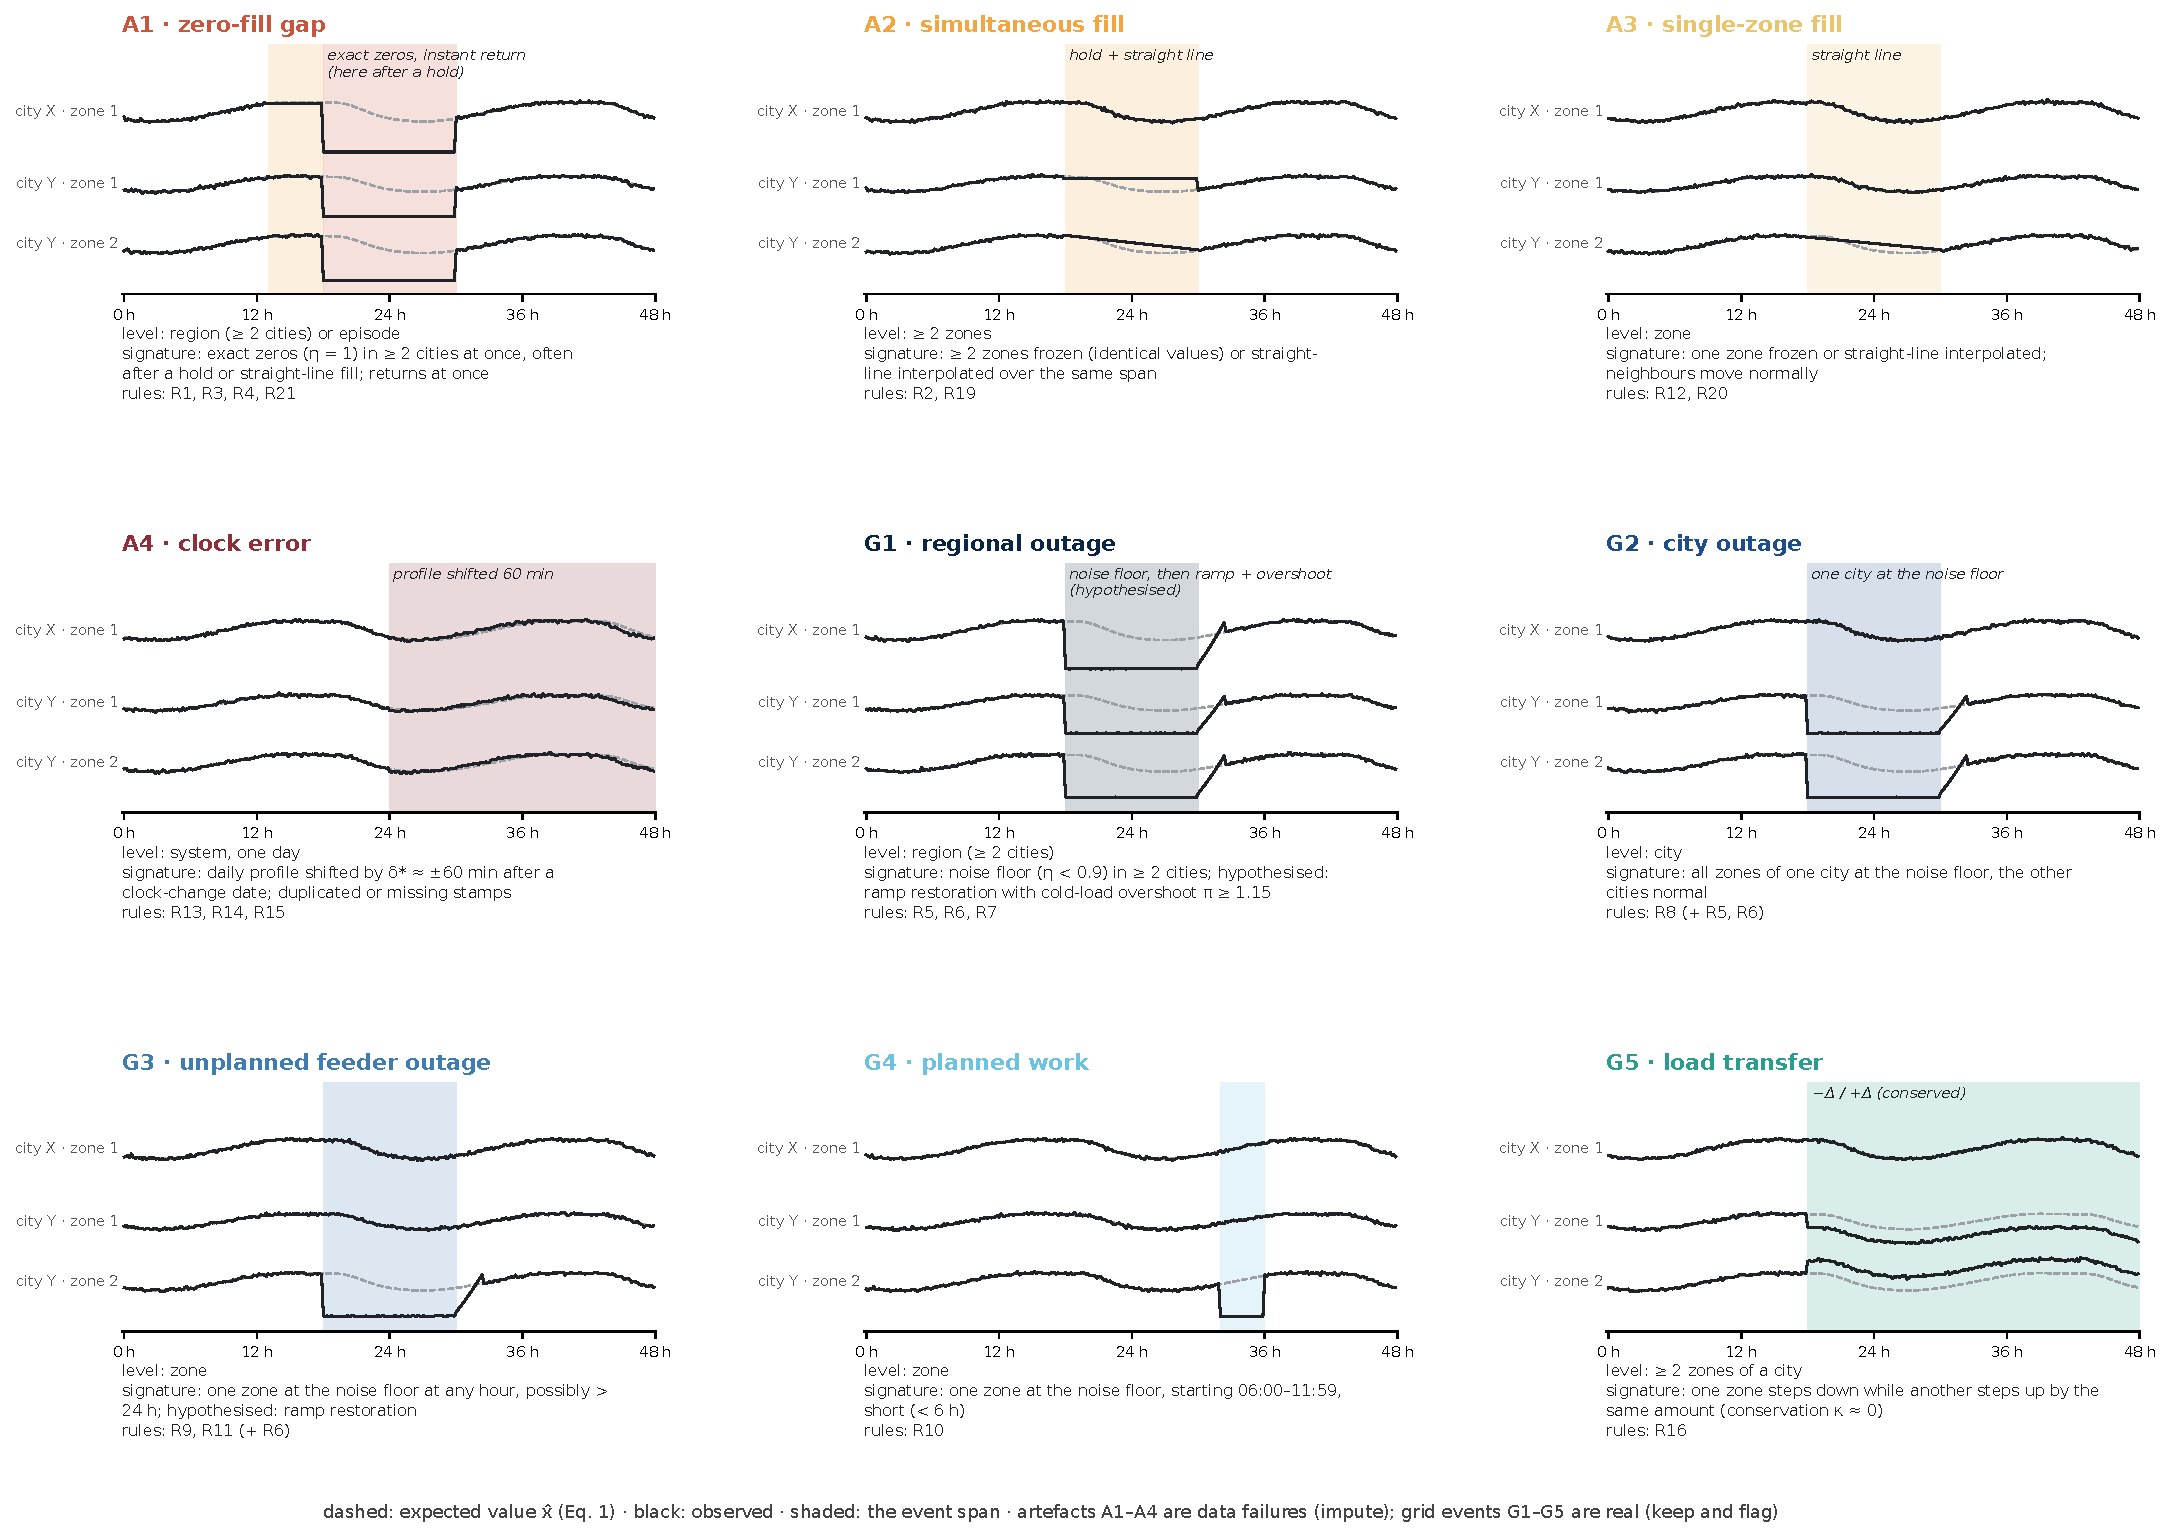
\includegraphics[width=\textwidth]{Figure_2}
\caption{Typology. Four data artefacts (A1--A4) and five grid events (G1--G5), each with a measurable signature at one level of the zone--city--region hierarchy and the rules that vote for it (schematic). Straight-line fills are part of A2 and A3.}
\label{fig:typology}
\end{figure}

% Method -- budget 1750 words. Plan (paper/OUTLINE.md): 4.1 overview (Fig 3); 4.2 states and signatures, Eqs (3)-(10); 4.3 rules (Table 4); 4.4 why the standard label model fails, Eq (11); 4.5 constrained label model, Eqs (12)-(13); 4.6 detector, Eqs (14)-(18); 4.7 end model and fusion, Eqs (19)-(20); 4.8 type-aware cleaning, Eq (21). Step 4.
\section{Method}\label{sec:method}

[To be written.]

% Experimental design -- budget 800 words (body text).
% Sources: docs/decisions.md D54, D56, D57, D60-D66, D68-D71, D76; docs/methods.md sections 6.1, 8, 9;
% src/inject.py (Table: DUR_H, _pick_zones, _place), src/benchmark.py (detection_metrics, step_auc, attribution_scores),
% src/label_model.py (ece), src/downstream.py (mase_scale, dm_test, dm_table); results/benchmark_v1/summary.json and
% dev_selection.json (8,526 events; 48 settings; development seeds 100-104).
\section{Experimental design}\label{sec:experiments}

Detection and attribution are measured on injected events, and the value of the catalogue downstream.

\subsection{Injection benchmark}\label{sec:injection}

Events are written into the real southern series inside \emph{clean zone-time}: zone-steps more than 53 steps from any rule state, after a 35-day burn-in and away from clock-change days. Table~\ref{tab:injection} lists the nine types; two untyped ones probe the detector where no rule fires. Events are placed in random type order, without overlap, until they cover 1, 3 or 7\% of the clean zone-steps.

The predictors are not retrained: cross-fitted on the real series, they predict every injected step from the other half of the real data. The rule engine, label model and end model are re-run on each injected dataset as on the real data. Every design choice was made on five development datasets (seeds 100--104). The 30 test datasets (three rates $\times$ seeds 0--9; 8,526 events) were used for no choice. Results refer to the test period, July 2023 to May 2024; the earlier period serves only to tune $\beta$.

\begin{table}[tbp]
\centering
\caption{Injected event types. Durations are log-uniform in the range, except G4 (uniform). $\xh$: expected value (Eq.~\eqref{eq:expected}); $U(a,b)$: uniform draw. Artefact signatures are copied from real episodes; grid-event signatures follow the hypothesised physics of Section~\ref{sec:typology}. Each event blocks its zones for $\pm 12$~h, and a multi-city event blocks the whole system for $\pm 3$~h. Clock errors (A4) and load transfers (G5) are not injected: their rules are calendar-gated or act on whole days.}
\label{tab:injection}
\footnotesize
\setlength{\tabcolsep}{4pt}
\begin{tabularx}{\textwidth}{@{}l L{3.6cm} l Y@{}}
\toprule
Type & Zones & Duration & Injected signature \\
\midrule
A1 & all zones of 2--3 cities & 0.5--24~h & exact zeros \\
A2 & 2 or more zones of one city (50\%), one city (25\%) or 2--3 cities (25\%) & 1--48~h & each zone held at its last value or interpolated by a straight line (50/50); a whole-city fill is followed by an A1 zero fill with probability 0.5 \\
A3 & one zone & 1--6~h & hold or straight-line fill \\
\midrule
G1 & all zones of 2 cities & 1--18~h & noise floor $\xh \cdot U(0, 0.03)$ with 0--30\% exact zeros; linear ramp of 20--90~min; overshoot $\omega \sim U(1.1, 1.5)$ decaying over 1--2~h \\
G2 & all zones of one city & 20~min--6~h & as G1 \\
G3 & one zone, any hour & 1--48~h & as G1 \\
G4 & one zone, start 06:00--11:59, 70\% at weekends & 1--6~h & noise floor as G1; ramp of 10--30~min; no overshoot \\
\midrule
U\_SHOCK & all zones of 2--3 cities & 0.5--4~h & scaled by $U(0.5, 0.8)$; no rule fires \\
U\_PARTIAL & one zone & 1--8~h & scaled by $U(0.10, 0.45)$, above the dead threshold \\
\bottomrule
\end{tabularx}
\end{table}

\subsection{Methods compared}\label{sec:compared}

Detection compares the rule engine alone, the main detector alone and the full method (rule items plus detector-only candidates) with three baselines: STL \cite{cleveland1990stl,seabold2010statsmodels} with a daily period, scored by the robust $z$-score of its remainder (Eq.~\eqref{eq:score}), and Isolation Forest \cite{liu2008iforest} and LOF \cite{breunig2000lof} on five per-step features of $\rho$. Ablations change one component of the main detector: the learned graph (removed), the predictor (LightGBM), the scales (raw band only), the hierarchy (flat zone score) or the event formation (untuned).

Every detector, baselines included, receives its own event formation: the best of the same 48 settings of $(w, q, g_{\max})$ by mean event F1 on the development datasets. Ablations inherit the main detector's setting; the no-graph ablation is also reported at its own. The main detector was chosen among four predictors by a criterion fixed beforehand: the development F1 of the rules plus its candidates. Baselines that were not run are discussed in Section~\ref{sec:discussion}.

Attribution compares the rules' majority vote, the label model, the end model and the fusion on the typed injected events that the full method detects.

\subsection{Metrics}\label{sec:metrics}

Detection is counted per event, without the point adjustment that inflates scores \cite{kim2022rigorous}. With $E$ the injected and $\hat{E}$ the predicted events,
\begin{equation}
\begin{gathered}
P = \frac{|\hat{E}^{*}|}{|\hat{E}|}, \qquad R = \frac{|E^{*}|}{|E|}, \qquad F_1 = \frac{2PR}{P + R}, \\
\hat{E}^{*} = \{\hat{e} \in \hat{E} : \hat{e} \cap E \neq \emptyset\}, \qquad E^{*} = \{e \in E : e \cap \hat{E} \neq \emptyset\},
\end{gathered}
\label{eq:eventf1}
\end{equation}
where $\hat{e} \cap E \neq \emptyset$ means that $\hat{e}$ overlaps an injected span in time, its restoration tail included; the zone-strict variant also requires a shared zone. Predictions that touch neither clean zone-time nor an injected span are not scored. A second view also ignores each method's own alarms on the uninjected series, as rule states already are. Step-wise AUC-PR and recall per type are also reported.

Attribution is scored by macro-F1 over the seven typed classes and by the expected calibration error \cite{guo2017calibration} of the arg-max probability over ten equal-width bins $B_b$:
\begin{equation}
\mathrm{ECE} = \sum_{b=1}^{10} \frac{|B_b|}{n} \left| \mathrm{acc}(B_b) - \mathrm{conf}(B_b) \right|.
\label{eq:ece}
\end{equation}

Forecasts $\hat{y}_{z,t}$ are scored on a set $S$ of zone-steps by the mean absolute scaled error \cite{hyndman2006mase},
\begin{equation}
\mathrm{MASE} = \frac{1}{|S|} \sum_{(z,t) \in S} a_{z,t}, \qquad a_{z,t} = \frac{|x_{z,t} - \hat{y}_{z,t}|}{s_z},
\label{eq:mase}
\end{equation}
where $s_z$ is the mean absolute one-day change of zone $z$ on normal training steps. Two strategies are compared by a Diebold--Mariano test \cite{diebold1995dm} on the loss summed over zones, $L_t = \sum_z a_{z,t}$:
\begin{equation}
d_t = L^{(1)}_t - L^{(2)}_t, \qquad \mathrm{DM} = \frac{\bar{d}}{\sqrt{\hat{\Omega}/n}}, \qquad
\hat{\Omega} = \hat{\gamma}_0 + 2 \sum_{k=1}^{h} \Big(1 - \frac{k}{h+1}\Big) \hat{\gamma}_k,
\label{eq:dm}
\end{equation}
where $\hat{\gamma}_k$ is the lag-$k$ autocovariance of $d_t$, with the Newey--West bandwidth \cite{newey1987hac} equal to the horizon $h$ because direct forecasts overlap. Outage counts are compared by the ratio of counted to true outage zone-hours and its log distance:
\begin{equation}
r = H / H^{\mathrm{true}}, \qquad \delta = |\log r|.
\label{eq:outage}
\end{equation}

\subsection{Downstream test}\label{sec:downstream}

On the southern system, the cleaning strategies S0--S3 (Section~\ref{sec:cleaning}) feed two forecasters, 1~h and 1~day ahead: a global LightGBM direct forecaster that also reads the event indicator, trained up to 31 December 2023, and a model-free reference (persistence at 1~h, seasonal naive at 1~day). Forecasts are scored from 1 January to 24 May 2024 against the recorded values, on zone-steps that every strategy treats as normal, and separately on those within two days after an anomalous state. Forecasting uses the real data and four injected test datasets; outage counts use all 30. Naive counting takes every flagged dead state and typed counting only those inside grid-event items; the truth is the injected G1--G4 spans.

\subsection{Transfer test}\label{sec:transfer}

Tetouan tests the method on a new system with nothing re-tuned. The rules, the label-model parameters (applied by one E-step), the architectures, the training settings and the event formation are frozen; the expected value, the score scales, the predictor weights and $\gamma_q$ (at the frozen percentile) are re-estimated from Tetouan's unlabelled series. With one city, G1 is not injected and multi-city types become city-wide. Thirty fresh injected datasets (three rates $\times$ 10 seeds) are scored over 2017.

\subsection{Statistics and reproducibility}\label{sec:statistics}

Results are mean $\pm$ standard deviation over the 10 seeds of each rate. Methods are compared by exact paired two-sided Wilcoxon signed-rank tests \cite{wilcoxon1945}: the smallest attainable $p$ is 0.002 over 10 seeds and $1.9 \times 10^{-9}$ over 30 datasets. The code uses Python, PyTorch \cite{paszke2019pytorch}, LightGBM 4.6.0 \cite{ke2017lightgbm} and scikit-learn \cite{pedregosa2011sklearn}; every injected dataset is regenerated from its rate and seed, and versions, settings and run times are given in the supplementary material.

% Results -- budget 1870 words (body text).
% Sources: docs/results_summary.md sections 5-11 (incl. 9.2d deep baselines, 10.1b outages and 10.2b forecasting on
% 30 datasets); docs/findings.md F01-F07, F16, F17, F21-F24, F30, F41-F47, F50, F51, F55-F59, F61-F63;
% results/catalogue_final/catalogue.csv (404 entries; rule-item confidence). Table rows generated from the result
% CSVs with half-up rounding (table5_detection.csv + deep_baselines/table_deep_baselines.csv, table6_attribution.csv,
% table8_forecasting.csv + forecast_all/forecast_summary.csv + dm_real.csv, transfer_tetouan/table9_detection.csv).
\section{Results}\label{sec:results}

\subsection{What the telemetry contains}\label{sec:res-telemetry}

The rule engine finds 327 items in the real data (126 dead, 155 fill, 33 clock and 13 transfer items), linked into 230 episodes. Straight-line fills, which the initial typology did not anticipate, are the most common fill mechanism: 85 fill items are pure straight lines, 54 pure holds and 16 mixed, and the first difference along a line is constant to about $10^{-14}$. Large events are compound episodes. In January 2023 (Fig.~\ref{fig:jan2023}) all 15 southern zones are filled at once, with holds in Laâyoune, Boujdour and one Foum El Oued zone and straight lines in the other six, and two days later all 15 zones are zero-filled for 13.7~h; the labels are A2, A2 and A1. In the episode of 31 March 2024 (Fig.~\ref{fig:mar2024}), held zones and zero-filled zones run side by side for 45.8~h: an acquisition state, not an electrical one.

No regional outage remains in the data. The regional-outage rule never fires, and all three multi-city dead events carry hold or straight-line evidence. The only regional-outage candidate, 16 July 2023, combines exact zeros in Boujdour and Foum El Oued with straight lines in every Laâyoune zone and is labelled an acquisition failure (A1, 0.93). The hypothesised restoration of grid events (Section~\ref{sec:typology}) is not supported either: 25 of the 117 southern dead runs (21\%) end in a straight line from the last zero to the first reading, so an apparent ramp is often an interpolation, and the learned evidence of the overshoot rule is almost nil ($\log(a/b) = 0.12$, against 1.8--4.8 for every other rule).

Clock errors follow the European, not the Moroccan, clock changes: the hour 02:00--02:50 is recorded twice on 30 October 2022 and 29 October 2023, and after the first date the daily profile is shifted by $\delta^* = -60$~min in all three cities.

Artefacts dominate the anomalous time. Counting every dead state as an outage gives 1,220.5 zone-hours in 117 runs; counting only the items typed as grid events gives 294.0 zone-hours in 79 runs, 4.15 times less. Zero fills (A1) alone account for 926.5 zone-hours.

\begin{figure}[tbp]
\centering
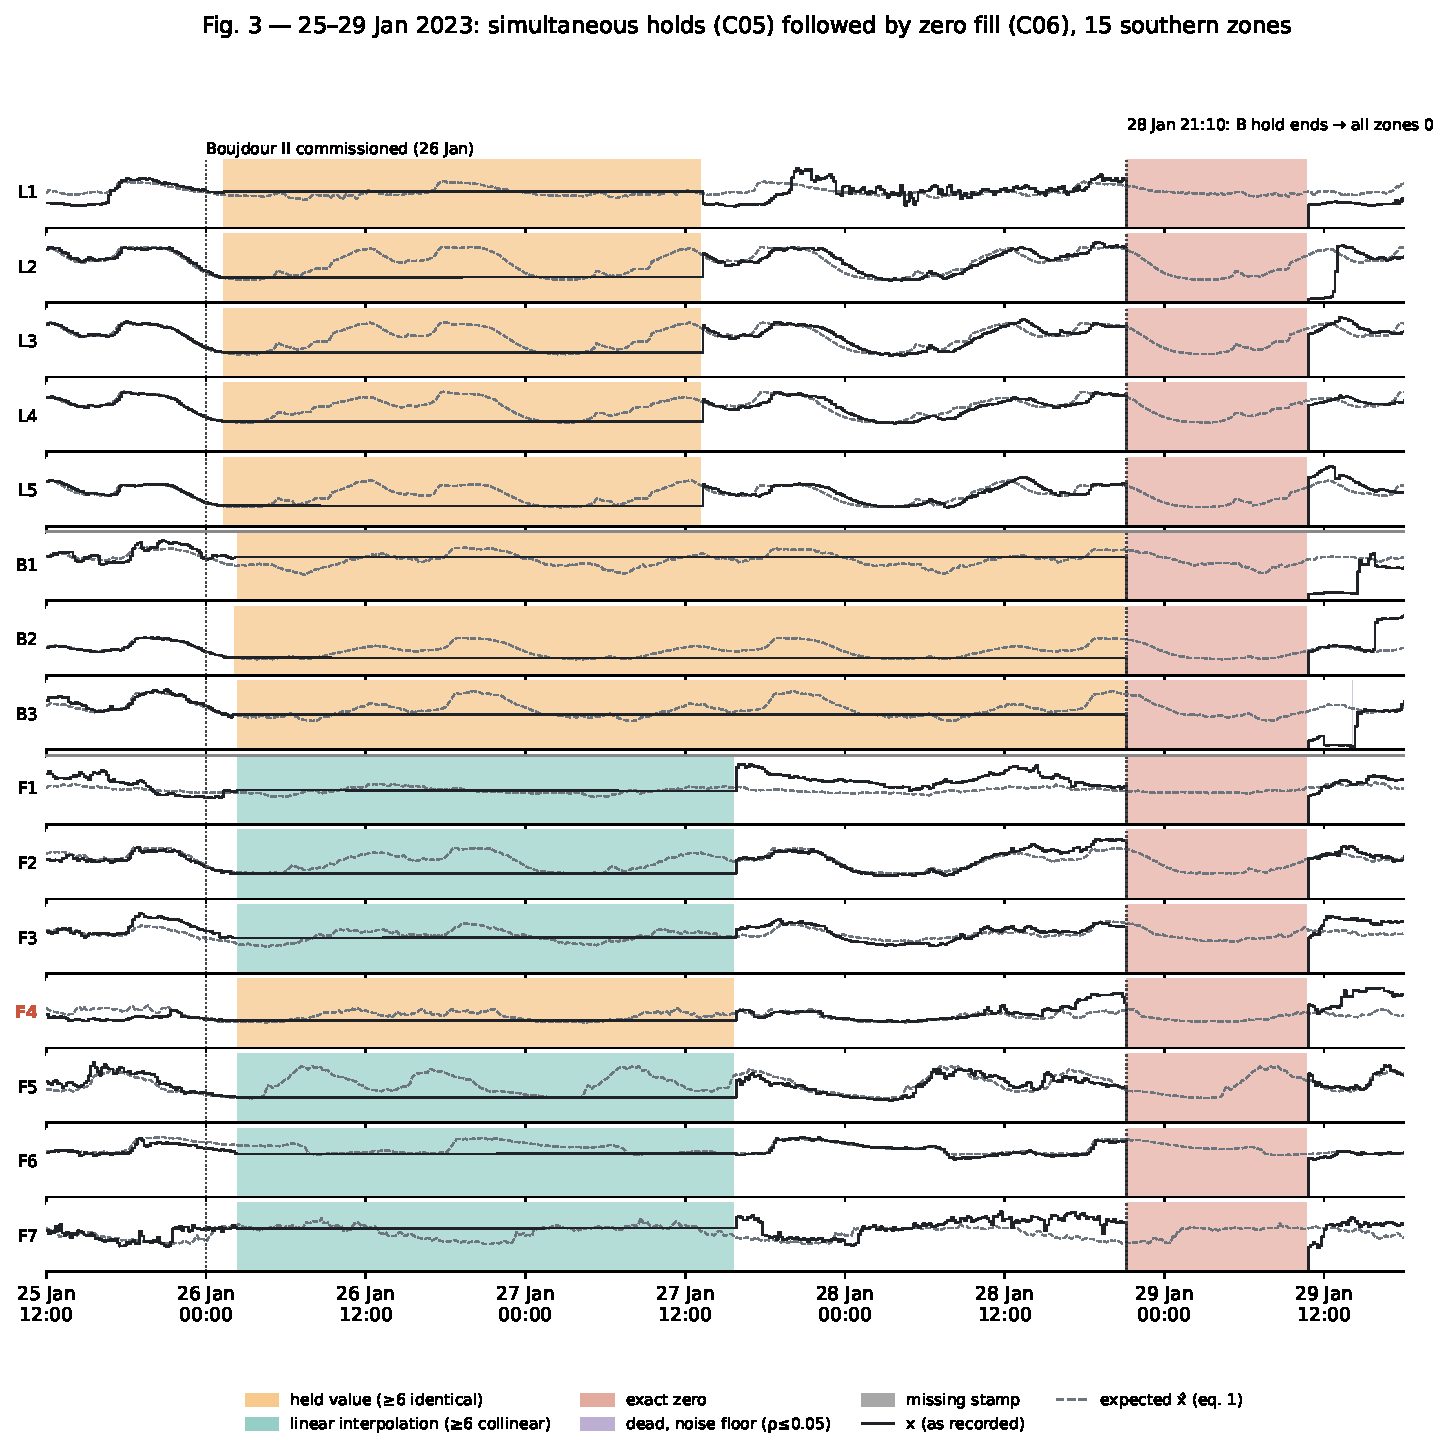
\includegraphics[width=\textwidth]{Figure_4}
\caption{The January 2023 acquisition episode (time stamps as recorded). Simultaneous holds (Laâyoune, Boujdour and F4) and straight-line fills (the other Foum El Oued zones) cover all 15 southern zones on 26--27 January; on 28 January all 15 zones are zero-filled for 13.7~h. Final labels A2, A2, A1.}
\label{fig:jan2023}
\end{figure}

\begin{figure}[tbp]
\centering
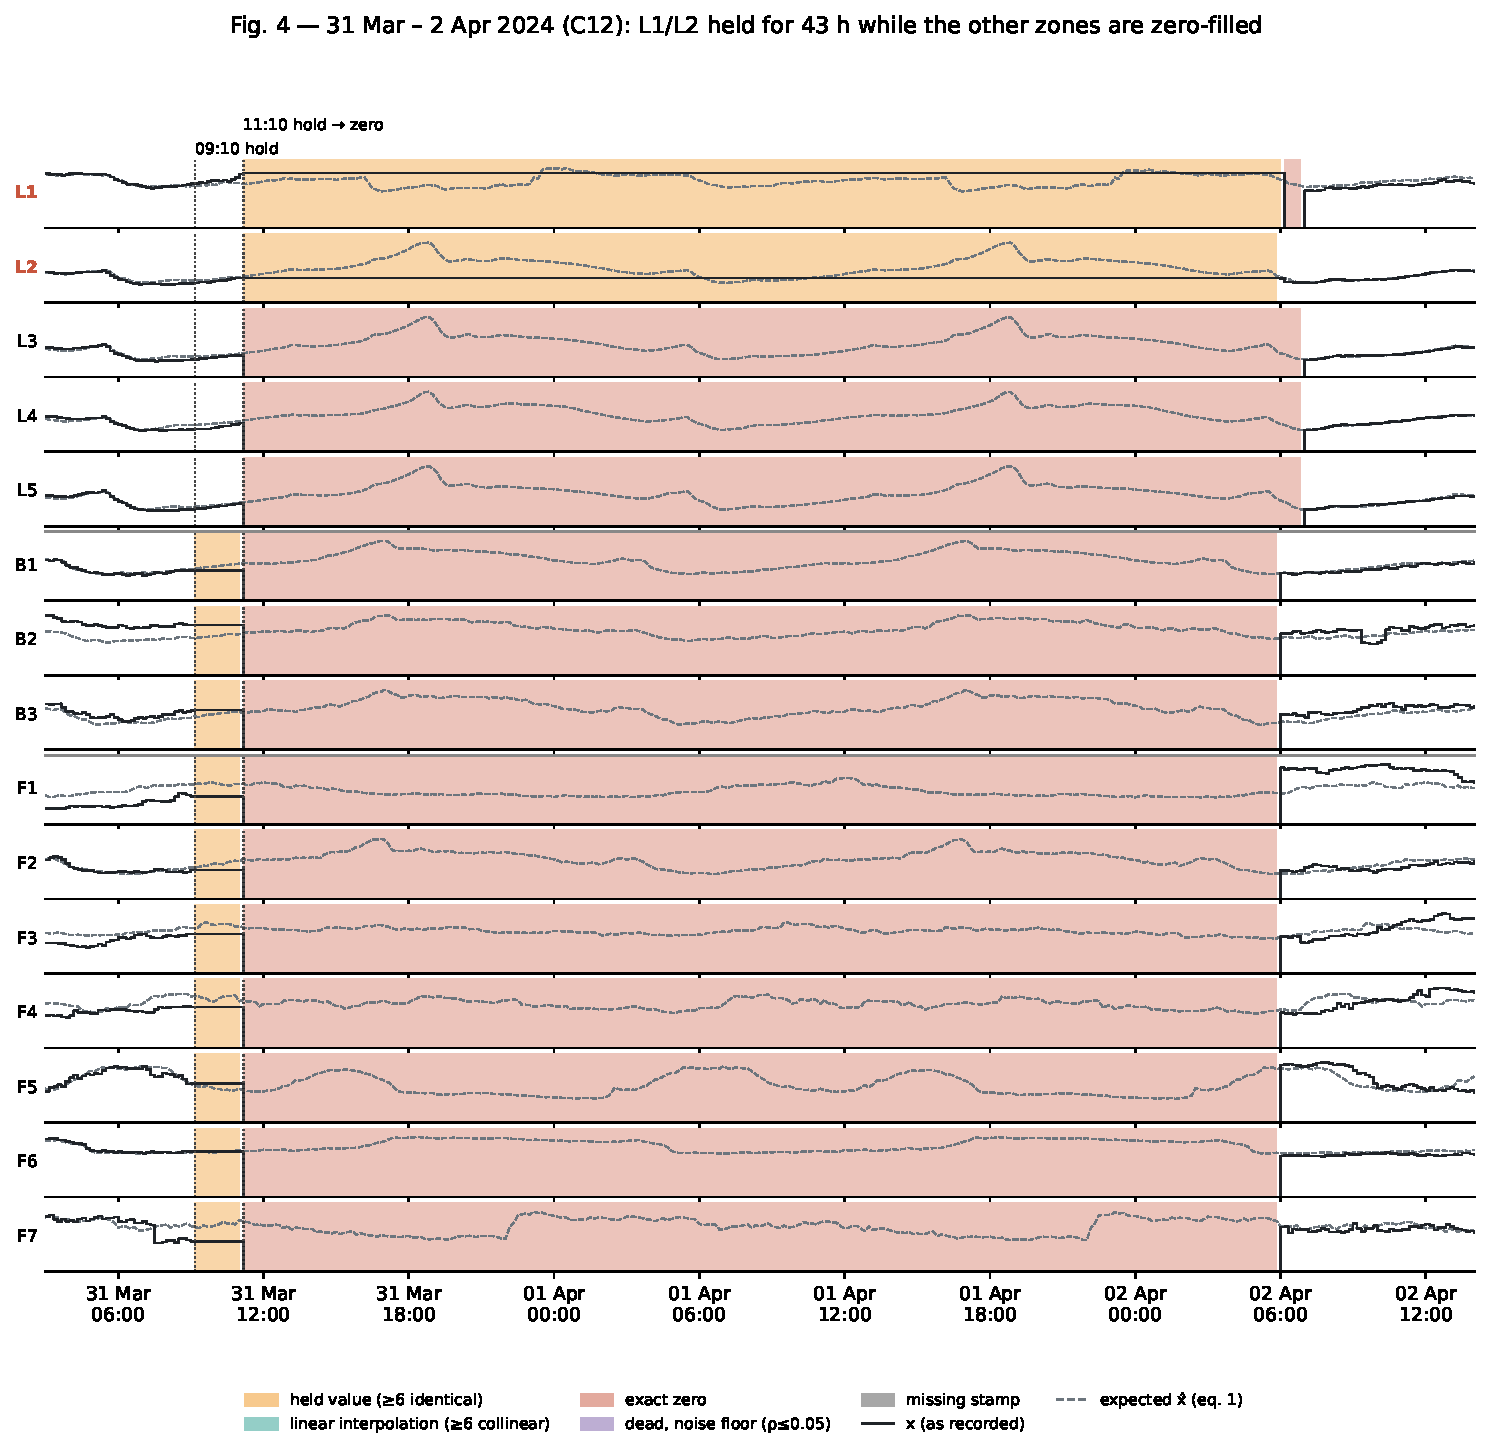
\includegraphics[width=\textwidth]{Figure_5}
\caption{The episode of 31 March -- 2 April 2024: Boujdour, Foum El Oued and L3--L5 are zero-filled while L1 and L2 are held. Final labels A2, A1, A2, G4; the last item, on L1, shows a limitation of the item-level label model (Section~\ref{sec:discussion}).}
\label{fig:mar2024}
\end{figure}

\subsection{Weak supervision on the real data}\label{sec:res-ws}

The constrained label model is stable where the standard one is not: its 20 restarts agree on every item, whereas restarts of the unconstrained Dawid--Skene model agree on as few as 62.7\% of the items (mean 83.2\%). On votes simulated from the fitted model, it recovers the true types with accuracy 0.922 and macro-F1 0.872 and is calibrated (ECE 0.033); the unconstrained model reaches 0.682, 0.493 and 0.276. Its labels agree with the rules' majority vote on 98.2\% of the items, but they come with probabilities: the mean confidence of the final rule-item labels is 0.937, and 13 items fall below 0.7.

The labels rest on the evidence one would expect. Dropping the straight-line rules changes 98.1\% of the fill labels and dropping the calendar rules 38.9\% of the dead labels, whereas dropping the simultaneity, restoration or single-zone rules changes none (supplementary material).

The released catalogue holds 404 entries: 327 rule items and 77 detector-only candidates (70 in the southern system, 7 in Marrakech). The rule items are labelled A3 98, G4 70, A2 57, G3 52, A4 14, A1 3, G2 1 and G5 1 (Table~\ref{tab:typology}), and 58 of the 70 southern candidates are untyped (N): partial drops, surges and short disturbances outside the typology.

\subsection{The residual hierarchy on the real data}\label{sec:res-hierarchy}

The hierarchy localises outages but not fills (Fig.~\ref{fig:hierarchy}). During the zero fills of January 2023, July 2023 and March 2024, the region part $g$ reaches robust $z$-scores of 218, 230 and 176, while a single-feeder outage moves only the zone part. All three multi-city dead items peak at the region level, and 92\% of the single-zone dead items at the zone level. Fills behave differently: a hold or a straight line drifts away from each zone's own expected path by a different amount, so the shared part stays small; only 17\% of the multi-city fills peak at the region level and 55\% of the city-wide fills at the city level. Fills are therefore found by their signatures, through the rules, rather than by the hierarchy, which makes the rules and the detector complementary.

\begin{figure}[tbp]
\centering
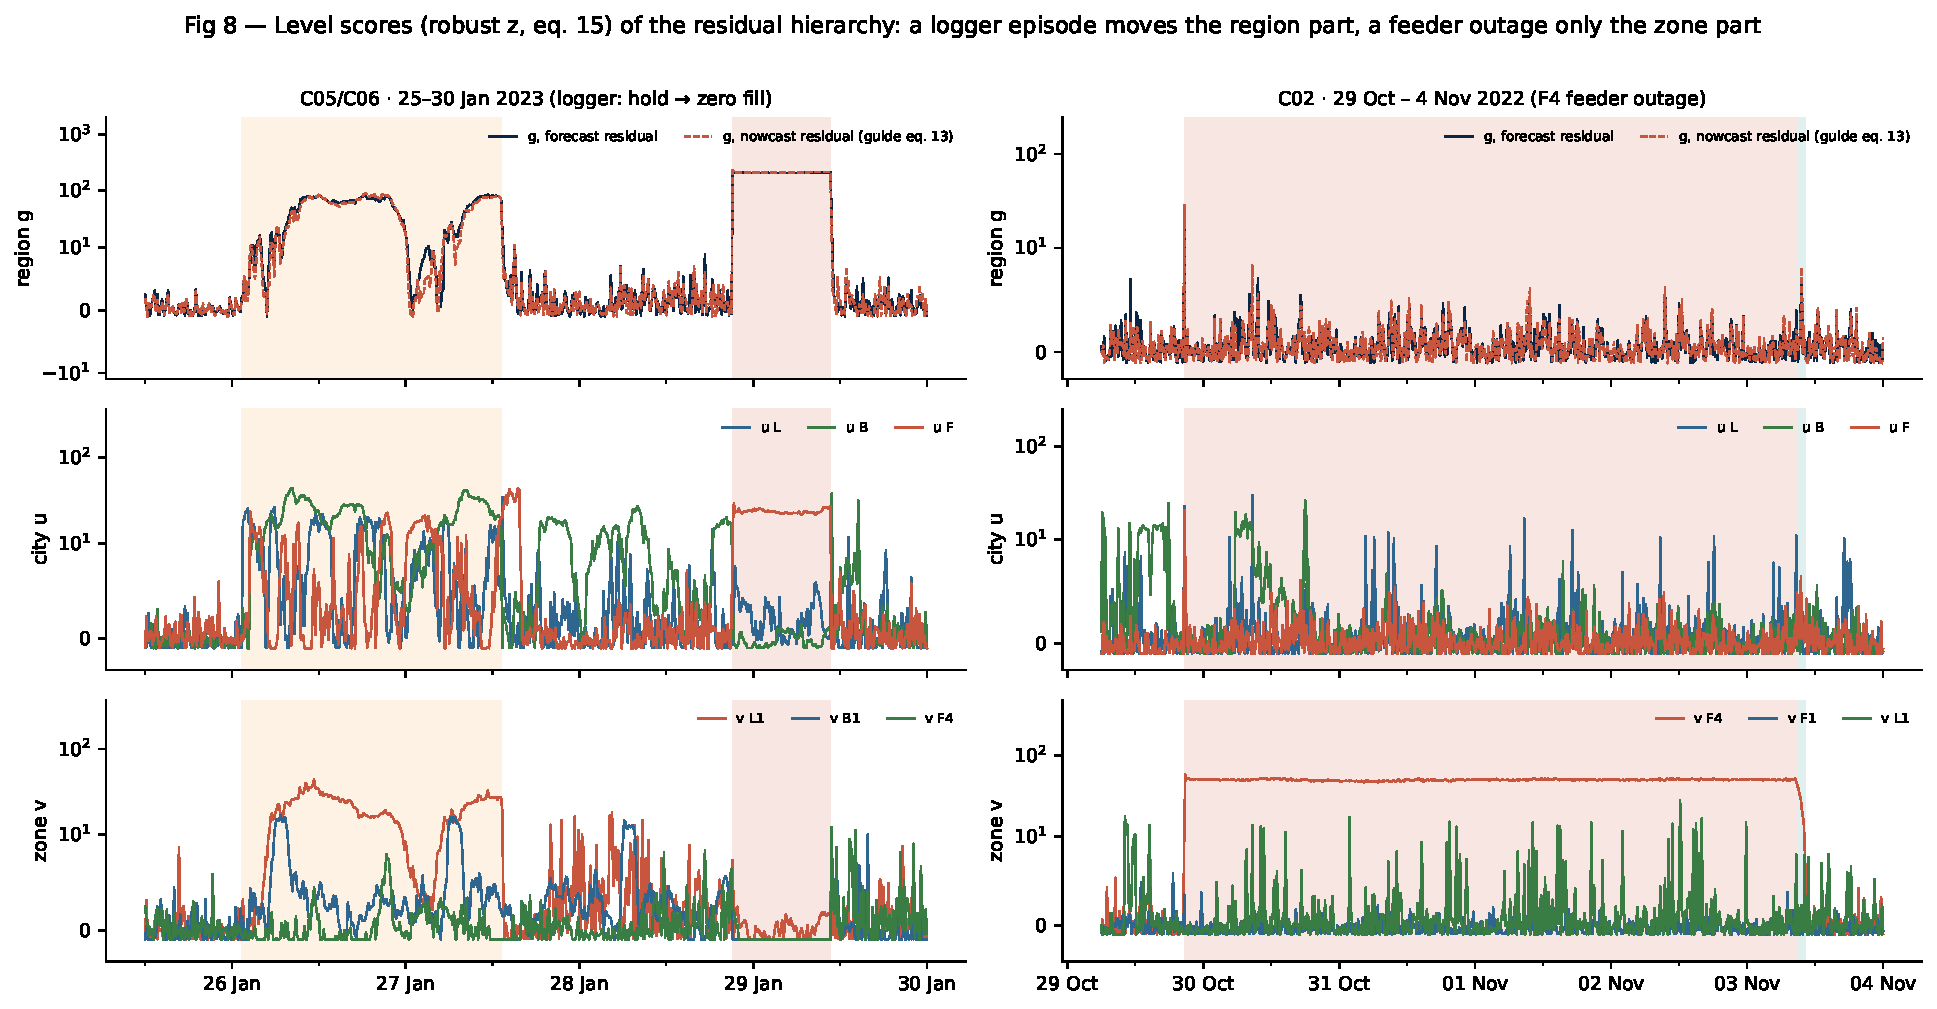
\includegraphics[width=\textwidth]{Figure_6}
\caption{Level scores (robust $z$-scores, Eq.~\eqref{eq:score}) of the residual hierarchy on the real data. During the January 2023 zero fill the region part $g$ reaches 218, while a feeder outage (F4, October 2022) moves only the zone part $v$. LightGBM residual; with the TCN-GAT residual, 73\% of the rule items peak at their structural level, against 71\%.}
\label{fig:hierarchy}
\end{figure}

\subsection{Detection on injected events}\label{sec:res-detection}

Fig.~\ref{fig:detection} and Table~\ref{tab:detection} compare the detectors. The rules alone reach event F1 0.86--0.90 at precision 1.00: they recall every injected type they were written for (city outages 0.90--0.94) and none of the untyped disturbances. The main detector is the best detector alone at 3\% and 7\% contamination (F1 0.813 and 0.854; Wilcoxon $p = 0.002$ against every other detector at 3\%, $p \le 0.020$ at 7\%); at 1\% (0.644) it is tied with the other residual detectors and STL ($p = 0.16$--$1.0$) and better than LOF and Isolation Forest. The deep baselines lose to the rules, to the main detector and to STL in every seed at every rate ($p = 0.002$): GDN reaches 0.37--0.71 and USAD 0.29--0.52. GDN finds 96--99\% of the multi-city zero gaps but fewer than 2\% of the single-zone fills, which are easy to forecast, and on clean data its forecasts are 7--14 times worse than the last value (supplementary material).

Adding the detector to the rules raises recall at every rate (0.82--0.84 against 0.76--0.81): it finds 5--30\% of the untyped city-wide shocks, 18--22\% of the partial drops and the city outages the rules miss. Its effect on F1 depends on how alarms are counted. If every alarm counts, the full method is worse than the rules at 1\% (0.721 against 0.863), equal at 3\% and better at 7\% (0.906 against 0.896, 10 of 10 seeds). If each method's own alarms on the uninjected series are excluded, as the rule states already are, it is better at every rate (0.90--0.91, $p = 0.002$). Under zone-strict matching it is worse at every rate: 25--75\% of the detector's extra alarms overlap an injected event in time but on other zones, because a zone left normal while its neighbours drop stands out at the city or region level.

The ablations (Fig.~\ref{fig:ablations}) locate the gain. Removing the learned graph leaves F1 equal or slightly higher ($+0.027$, $+0.004$ and $+0.003$): the graph adds interpretability, through the learned cross-city dependencies, but no detection skill. The tuned event formation contributes most ($-0.28$, $-0.14$ and $-0.02$ without it), followed by the multi-scale bands at low contamination ($-0.05$ and $-0.04$ at 1 and 3\%). A flat residual instead of the region--city--zone hierarchy does not lower F1 consistently: the hierarchy serves localisation, not detection. Smoothing costs timing: the median onset error is 140--168~min, against 60--70~min for STL.

\begin{figure}[tbp]
\centering
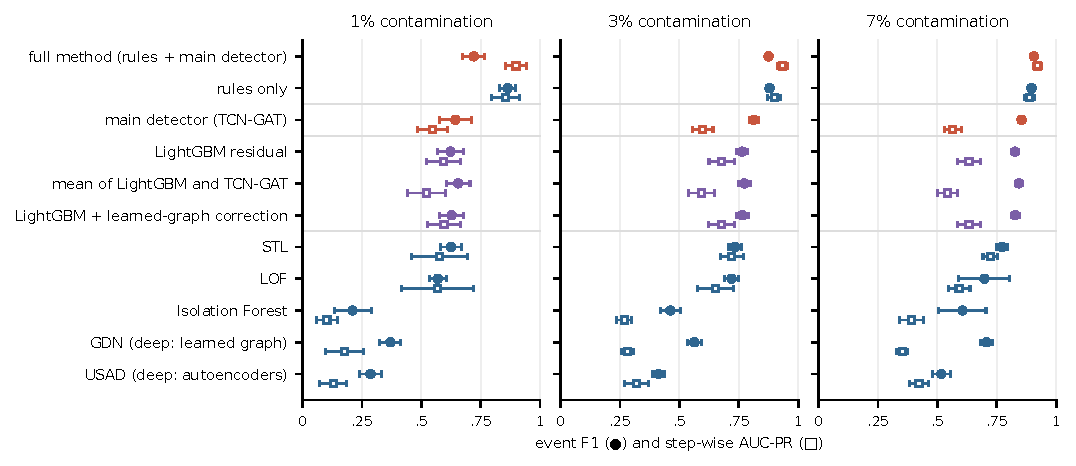
\includegraphics[width=\textwidth]{Figure_7}
\caption{Detection on injected events, test period: event F1 (circles, Eq.~\eqref{eq:eventf1}) and step-wise AUC-PR (squares), mean $\pm$ s.d. over 10 seeds at 1, 3 and 7\% contamination. Red: the full method and the main detector; purple: other predictors in the same residual detector; blue: the rules and the baselines, classical and deep. The ablations of the main detector are in Fig.~\ref{fig:ablations}.}
\label{fig:detection}
\end{figure}

\begin{table}[tbp]
\centering
\caption{Detection on injected events: the views that Fig.~\ref{fig:detection} does not show. Test period, mean over 10 seeds at 1 / 3 / 7\% contamination. Own background excluded: each method's own alarms on the uninjected series are not scored. Zone-strict: a match also requires a shared zone. Real-data alarms: alarms of the detector alone on the uninjected southern series (full method, i.e. the rules and the main detector: its detector-only candidates). LightGBM residual: the main detector with a LightGBM predictor and its own event formation.}
\label{tab:detection}
\scriptsize
\setlength{\tabcolsep}{3.5pt}
\begin{tabular}{@{}l c c c c r@{}}
\toprule
& & & F1, own background & Zone-strict & Real-data \\
Method & Precision & Recall & excluded & F1 & alarms \\
\midrule
Full method & 0.65/0.92/0.98 & 0.82/0.83/0.84 & 0.90/0.91/0.91 & 0.63/0.78/0.81 & 70 \\
Rules alone & 1.00/1.00/1.00 & 0.76/0.79/0.81 & 0.86/0.88/0.90 & 0.86/0.87/0.88 & -- \\
\midrule
Main detector & 0.58/0.89/0.98 & 0.73/0.75/0.76 & 0.82/0.84/0.85 & 0.62/0.78/0.81 & 191 \\
LightGBM residual & 0.57/0.82/0.96 & 0.69/0.72/0.73 & 0.79/0.82/0.83 & 0.61/0.74/0.77 & 152 \\
\midrule
STL & 0.64/0.87/0.97 & 0.62/0.64/0.64 & 0.74/0.76/0.76 & 0.61/0.71/0.71 & 178 \\
LOF & 0.51/0.77/0.91 & 0.66/0.68/0.57 & 0.71/0.76/0.70 & 0.55/0.69/0.64 & 263 \\
Isolation Forest & 0.14/0.37/0.65 & 0.48/0.63/0.57 & 0.39/0.63/0.65 & 0.17/0.42/0.53 & 457 \\
GDN & 0.27/0.52/0.78 & 0.60/0.62/0.65 & 0.68/0.70/0.74 & 0.29/0.46/0.57 & 366 \\
USAD & 0.23/0.49/0.76 & 0.38/0.36/0.39 & 0.43/0.45/0.48 & 0.23/0.35/0.41 & 243 \\
\bottomrule
\end{tabular}
\end{table}

\begin{figure}[tbp]
\centering
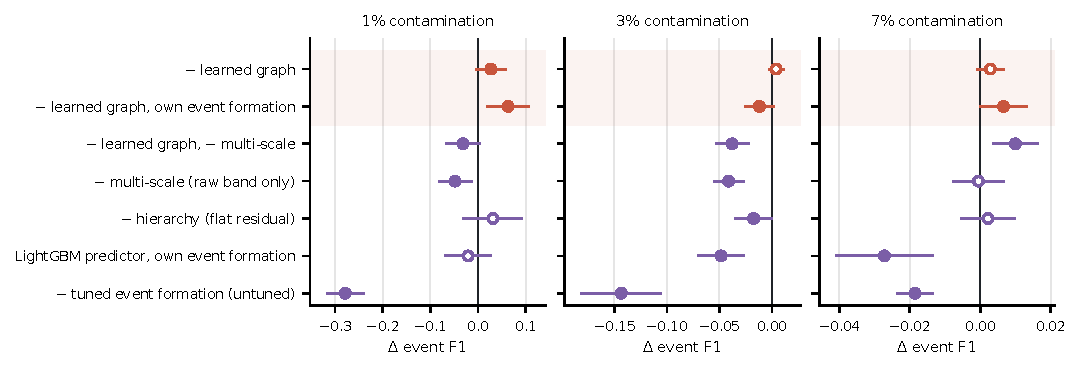
\includegraphics[width=\textwidth]{Figure_8}
\caption{Ablations of the main detector: change in event F1 relative to the main detector (mean $\pm$ s.d. of the per-seed differences; filled markers: Wilcoxon $p < 0.05$). The learned-graph ablation (shaded) leaves F1 equal or slightly higher; the multi-scale bands and the tuned event formation carry the gain.}
\label{fig:ablations}
\end{figure}

\subsection{Attribution}\label{sec:res-attribution}

On the injected events that the full method detects, every labeller reaches macro-F1 0.85--0.94 (Table~\ref{tab:attribution}). The label model does not beat the rules' majority vote on these signatures (0.900--0.934 against 0.913--0.940), the fusion matches both (0.906--0.944), and the end model alone is weaker at low contamination. What weak supervision adds is a calibrated probability for each label: the expected calibration error of the label model and of the fusion stays between 0.07 and 0.10 without recalibration (Fig.~\ref{fig:attribution}b). End to end, 0.90--0.95 of the typed injected events are both detected and correctly typed.

One confusion dominates (Fig.~\ref{fig:attribution}a): at 3\%, 44 of 160 zero-fill gaps (A1) are labelled regional outages (G1). The injected gaps drop to exactly zero in several cities at once, the simultaneity rules vote for a regional event, and nothing else separates the two; the real multi-city gaps also carry fill evidence, which the injector does not copy. Without the simultaneity rules the label model's A1 accuracy would rise from 0.70 to 0.83 and its macro-F1 from 0.914 to 0.941; we report this but do not adopt it, because it was observed on the test seeds. The other classes reach F1 0.86--0.99; feeder outages are sometimes taken for planned work (15 of 123).

\begin{table}[tbp]
\centering
\caption{Attribution of the injected events detected by the full method (test period; macro-F1 over the seven typed classes, mean $\pm$ s.d. over 10 seeds, and the mean expected calibration error, Eq.~\eqref{eq:ece}). Majority vote gives no probabilities.}
\label{tab:attribution}
\footnotesize
\setlength{\tabcolsep}{2.5pt}
\begin{tabular}{@{}l ccc ccc@{}}
\toprule
& \multicolumn{3}{c}{Macro-F1} & \multicolumn{3}{c}{ECE} \\
\cmidrule(lr){2-4}\cmidrule(l){5-7}
Labeller & 1\% & 3\% & 7\% & 1\% & 3\% & 7\% \\
\midrule
Majority vote & 0.940 $\pm$ 0.054 & 0.921 $\pm$ 0.029 & 0.913 $\pm$ 0.015 & -- & -- & -- \\
Label model $q$ & 0.934 $\pm$ 0.055 & 0.914 $\pm$ 0.029 & 0.900 $\pm$ 0.017 & 0.068 & 0.089 & 0.099 \\
End model $f$ & 0.845 $\pm$ 0.071 & 0.874 $\pm$ 0.025 & 0.902 $\pm$ 0.018 & 0.107 & 0.078 & 0.061 \\
Fusion $p$ & 0.944 $\pm$ 0.037 & 0.919 $\pm$ 0.023 & 0.906 $\pm$ 0.019 & 0.074 & 0.090 & 0.100 \\
\bottomrule
\end{tabular}
\end{table}

\begin{figure}[tbp]
\centering
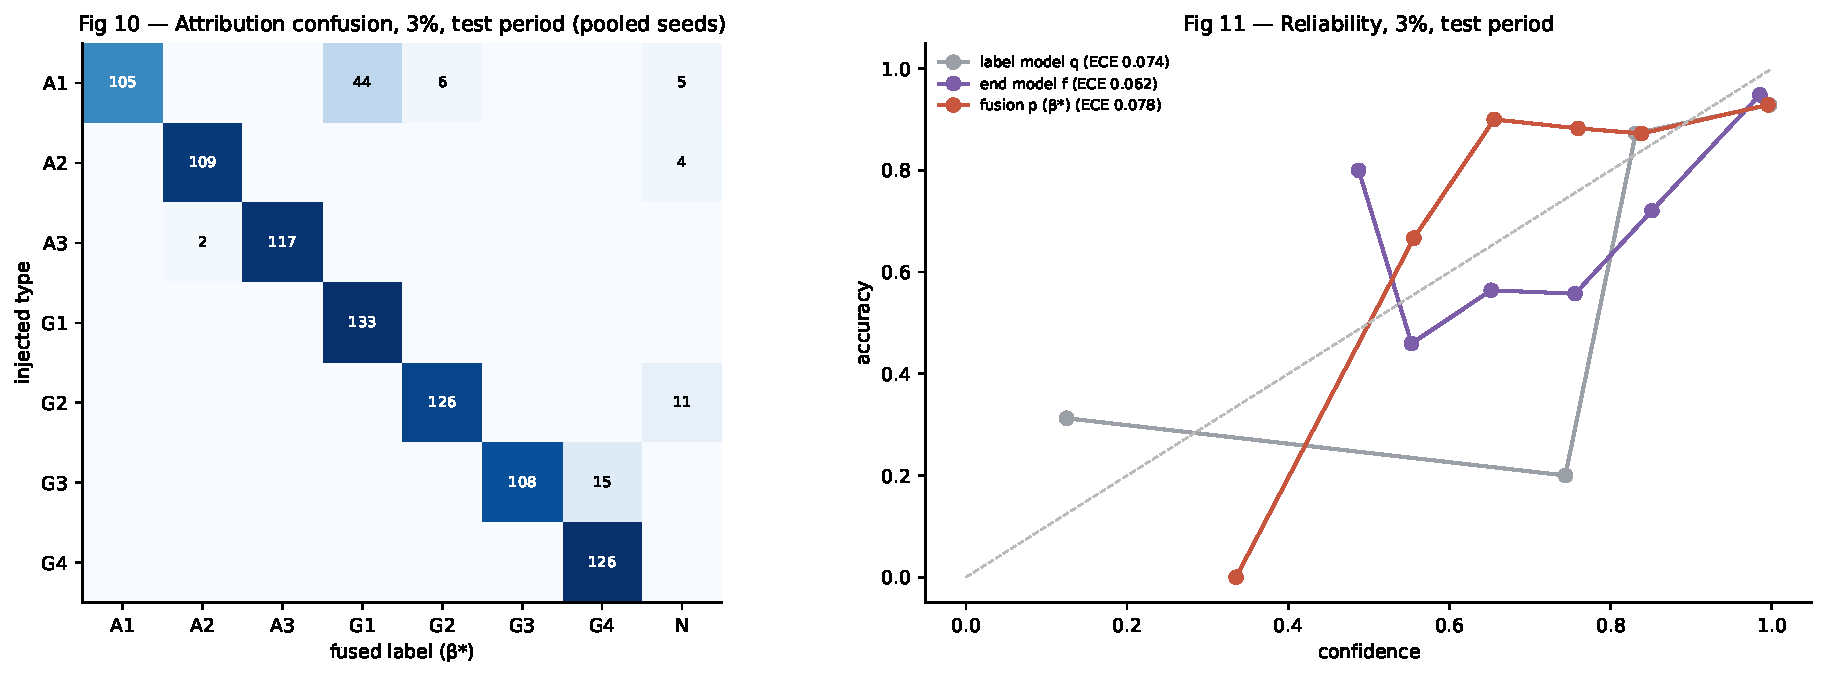
\includegraphics[width=\textwidth]{Figure_9}
\caption{Attribution on injected events (3\%, test period, seeds pooled): (a) confusion of the injected type and the fused label; (b) reliability of the label model $q$, the end model $f$ and the fusion $p$.}
\label{fig:attribution}
\end{figure}

\subsection{Outage statistics and forecasting}\label{sec:res-downstream}

On the injected data, where the truth is known, naive counting overstates outage zone-hours $1.88 \pm 0.32$ times and typed counting $1.26 \pm 0.24$ times (Fig.~\ref{fig:downstream}c). Typed counting is closer to the truth in all 30 datasets ($p = 1.9 \times 10^{-9}$) and recovers 99.8\% of the true outage zone-steps, and 99.98\% of its remaining excess lies inside injected zero-fill gaps: it is the A1-to-G1 confusion of Section~\ref{sec:res-attribution}, and nothing else. Interpolation (S1) erases outages from the record altogether. On the real data, the two counts differ 4.15-fold (Section~\ref{sec:res-telemetry}).

Type-aware cleaning also gives the most accurate forecasts when the forecaster reads the event indicator (Table~\ref{tab:downstream}, Fig.~\ref{fig:downstream}a--b). On the real data, the LightGBM day-ahead MASE after an anomaly falls from 1.501 (raw) and 1.233 (interpolated) to 1.061, 14\% below interpolation; the gain is significant at 1~h (DM $p < 0.001$) but not day-ahead ($p = 0.22$), because a few multi-zone events carry it. On the 30 injected datasets, S2 gives the lowest LightGBM error in 28--30 of them (Wilcoxon $p \le 5 \times 10^{-6}$) and comes within 0.006 MASE of the oracle S3. Over all test steps the effect is small, about 1\% against interpolation on the real data, because anomalies are rare. With the model-free reference the order changes: persistence and seasonal naive copy a kept outage into the next hour or day, so interpolation forecasts better (S1 beats S2 in all 30 datasets at 1~h), at the price of erasing the outages from the statistics.

\begin{table}[tbp]
\centering
\caption{Forecast error (MASE, Eq.~\eqref{eq:mase}) by cleaning strategy, test period 1 January -- 24 May 2024. After: steps within two days after an anomalous state in the zone; all: every scored step. Real data: S0 / S1 / S2 and the Diebold--Mariano $p$ of S1 against S2. Injected: S0 / S1 / S2 / S3, mean over the 30 test datasets, and the number of datasets in which S2 beats S1 with the Wilcoxon $p$ (S1 is better when the number is below 15).}
\label{tab:downstream}
\scriptsize
\setlength{\tabcolsep}{4pt}
\begin{tabular}{@{}l l l c c c c@{}}
\toprule
& & & \multicolumn{2}{c}{Real data} & \multicolumn{2}{c}{Injected data (30 datasets)} \\
\cmidrule(lr){4-5}\cmidrule(l){6-7}
Forecaster & Horizon & Steps & S0 / S1 / S2 & DM $p$ & S0 / S1 / S2 / S3 & S2 better (p) \\
\midrule
LightGBM & 1 h & after & 0.656/0.661/0.613 & $<$0.001 & 0.696/0.636/0.625/0.619 & 29 (4e-6) \\
LightGBM & 1 h & all & 0.654/0.657/0.654 & 0.019 & 0.653/0.625/0.625/0.620 & 28 (4e-6) \\
LightGBM & 1 day & after & 1.501/1.233/1.061 & 0.22 & 1.295/1.140/1.058/1.052 & 29 (5e-7) \\
LightGBM & 1 day & all & 1.140/1.115/1.102 & 0.25 & 1.174/1.076/1.052/1.051 & 29 (3e-6) \\
\midrule
Naive & 1 h & after & 1.081/1.059/1.052 & 0.44 & 0.995/0.920/0.939/0.923 & 0 (2e-9) \\
Naive & 1 day & after & 2.220/1.553/1.278 & 0.16 & 2.036/1.377/1.499/1.448 & 10 (6e-4) \\
\bottomrule
\end{tabular}
\end{table}

\begin{figure}[tbp]
\centering
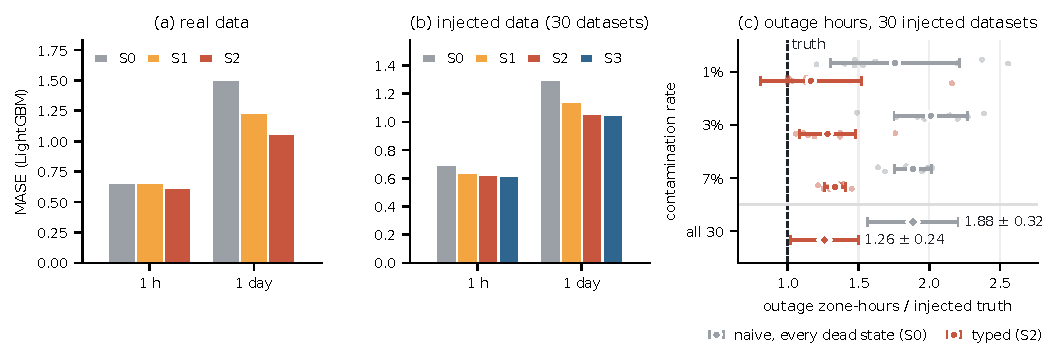
\includegraphics[width=\textwidth]{Figure_10}
\caption{Downstream test. LightGBM forecast error (MASE) by cleaning strategy on test steps within two days after an anomaly, (a) real data and (b) injected data (mean of 30 datasets); test period 1 January -- 24 May 2024. (c) Outage zone-hours relative to the injected truth under naive (S0) and typed (S2) counting on the 30 injected datasets (points: seeds; markers: mean $\pm$ s.d.). Interpolation (S1) reports no outage.}
\label{fig:downstream}
\end{figure}

\subsection{Transfer to Tetouan}\label{sec:res-transfer}

Tetouan tests the frozen method on another city and year (Fig.~\ref{fig:transferprotocol}). On the real 2017 series the rules raise no dead or fill item, and the four clock-change dates they examine are all labelled normal; the main detector raises 7 alarms in the year, 0.20 per zone-month, against 72 for Isolation Forest. On the injected datasets the full method reaches event F1 0.945, 0.919 and 0.890 at 1, 3 and 7\% contamination, at precision 0.98--1.00 (Table~\ref{tab:tetouan}, Fig.~\ref{fig:tetouan}a), and beats the rules alone (0.856--0.861) in every seed at every rate ($p = 0.002$). The main detector alone is the best detector at 1\% (0.857). At 3\% LightGBM and STL overtake it ($p = 0.002$ and 0.004), and at 7\% LightGBM and Isolation Forest ($p = 0.006$ and 0.002): on one year of three zones, the neural predictor forecasts four times worse than LightGBM (MAE 0.045 against 0.011).

Attribution transfers except for one class (Fig.~\ref{fig:tetouan}b). The frozen label model reaches macro-F1 0.77--0.79, and 0.95--0.98 without A1: 348 of 417 injected zero-fill gaps are read as city outages, with confidence above 0.98. In Morocco, a gap is told from an outage by its zeros in several cities at once; in a single city this evidence cannot exist.

\begin{figure}[tbp]
\centering
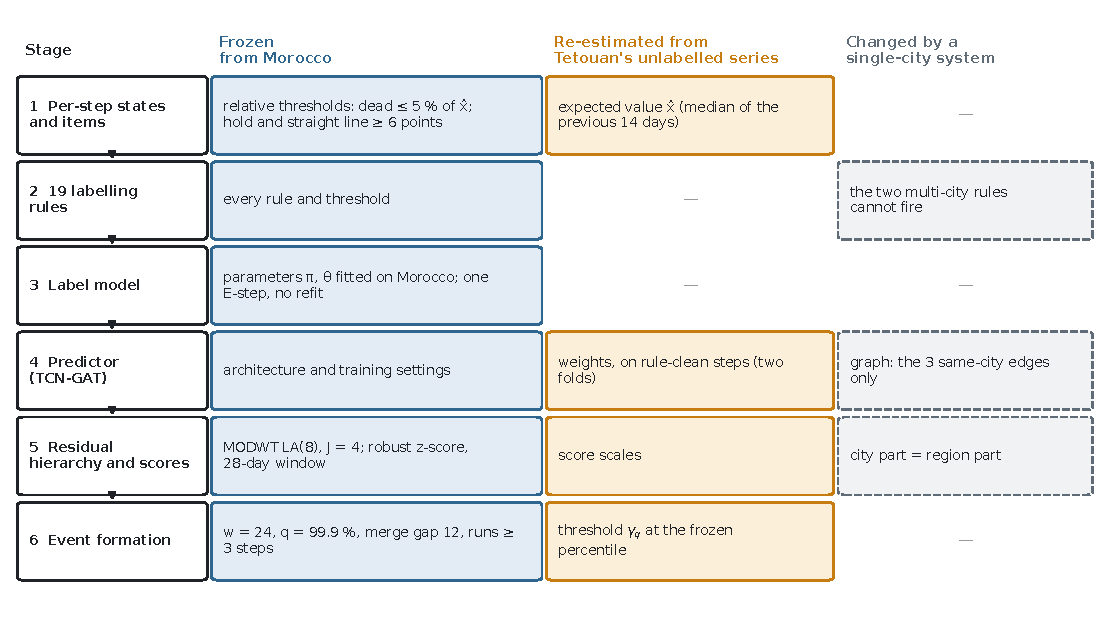
\includegraphics[width=\textwidth]{Figure_11}
\caption{Transfer protocol: what is frozen from the Moroccan system, what is re-estimated from Tetouan's unlabelled series, and what a single-city system changes.}
\label{fig:transferprotocol}
\end{figure}

\begin{table}[tbp]
\centering
\caption{Transfer to Tetouan without re-tuning (event F1 in Fig.~\ref{fig:tetouan}a). Injected data: mean over 10 seeds at 1 / 3 / 7\% contamination. Full method: the rules and the main detector. No graph: the main detector without the learned graph (same event formation). Real alarms: items or alarms raised on the real 2017 series (clock items labelled N excluded).}
\label{tab:tetouan}
\scriptsize
\setlength{\tabcolsep}{4pt}
\begin{tabular}{@{}l c c c r@{}}
\toprule
Method & Precision & Recall & AUC-PR & Real alarms \\
\midrule
Full method & 0.98 / 1.00 / 1.00 & 0.91 / 0.85 / 0.80 & 0.95 / 0.95 / 0.95 & 7 \\
Rules alone & 1.00 / 1.00 / 1.00 & 0.75 / 0.76 / 0.75 & 0.88 / 0.89 / 0.88 & 0 \\
\midrule
Main detector & 0.98 / 1.00 / 1.00 & 0.76 / 0.66 / 0.57 & 0.75 / 0.66 / 0.69 & 7 \\
Main detector, no graph & 0.99 / 1.00 / 1.00 & 0.72 / 0.65 / 0.55 & 0.52 / 0.57 / 0.61 & 9 \\
LightGBM residual & 0.75 / 0.98 / 1.00 & 0.79 / 0.78 / 0.62 & 0.84 / 0.82 / 0.83 & 15 \\
\midrule
STL & 0.77 / 0.97 / 1.00 & 0.72 / 0.72 / 0.59 & 0.80 / 0.78 / 0.81 & 13 \\
Isolation Forest & 0.35 / 0.61 / 0.90 & 0.81 / 0.81 / 0.73 & 0.42 / 0.54 / 0.66 & 72 \\
LOF & 0.76 / 0.90 / 0.70 & 0.73 / 0.62 / 0.12 & 0.66 / 0.59 / 0.29 & 11 \\
\bottomrule
\end{tabular}
\end{table}

\begin{figure}[tbp]
\centering
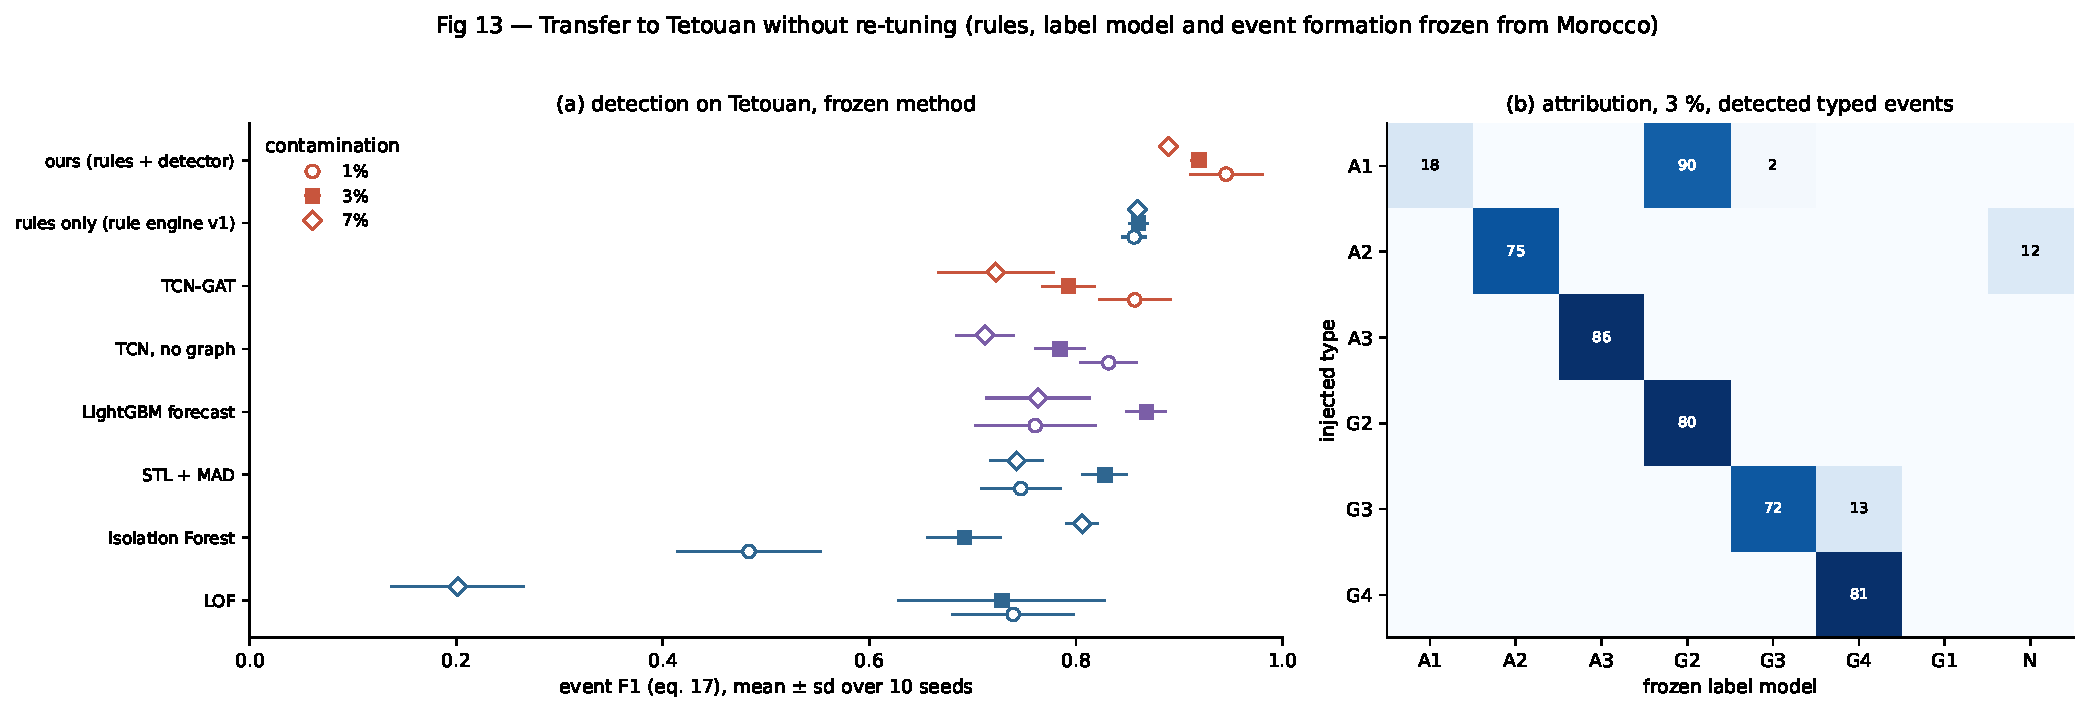
\includegraphics[width=\textwidth]{Figure_12}
\caption{Transfer to Tetouan without re-tuning: (a) event F1 of every method at 1, 3 and 7\% contamination; (b) confusion of the frozen label model at 3\%. City-wide zero gaps (A1) are read as city outages (G2).}
\label{fig:tetouan}
\end{figure}

% Discussion -- budget 700 words. Plan (paper/OUTLINE.md): 7.1 RQ and H answers (Table 9); 7.2 implications for distribution operators; 7.3 limitations and threats to validity. Step 7.
\section{Discussion}\label{sec:discussion}

[To be written.]

% Conclusions -- budget 250 words. Plan (paper/OUTLINE.md): V1-V5 summary; future work. Step 10.
\section{Conclusions}\label{sec:conclusions}

[To be written.]

% Declarations (wording to be checked against the guide for authors before submission).
\section*{Data and code availability}
The UCI datasets analysed in this study are publicly available \cite{bensalah2025uci,salam2018uci}. The code, the typed event catalogue and all results will be made publicly available. [Repository and archive identifiers to be added.]

\section*{CRediT authorship contribution statement}
[To be added by the authors.]

\section*{Declaration of competing interest}
The authors declare that they have no known competing financial interests or personal relationships that could have appeared to influence the work reported in this paper.

\section*{Funding}
[To be added by the authors.]


\bibliographystyle{elsarticle-num}
\bibliography{references}

\end{document}
